\chapter{Experiments}

Precision and recall are favoured values in image retrieval. Precision is the fraction of relevant retrieved objects and all the retrieved objects. Recall is the ratio of relevant retrieved objects to all the relevant objects. Although, many retrieval system is capable to return a ranked list of the retrieved objects, precision and recall ignore this information. Thus, the trained models are evaluated with the nowadays very popular mean average precision (mAP) metric. In particular, a descending sorted list will be created for every company, based on the probabilities of being logos from the specific brand on given positions of the images. Firstly the precision curve as a function of recall is acquired for every list. The average precision is then calculated as the area under the precison-recall curve. The average of these values gives the mean average precision.
All the mentioned results will be calculated with the evaluation implementation of py-faster-rcnn \cite{Girshick2017} \cite{NIPS2015_5638}.

\section{Training with Synthetic Data}

\subsection{FlickrBelgaLogos dataset}

A dataset, which is annotated manually, may contain logos, which stay unannotated. If a system is evaluated on such a dataset, and finds the unannotated logo, it counts as false positive detection. Thus, a synthetic dataset, called FlickrBelgalogos \cite{letessier2012scalable} is created for evaluation purpose, by pasting the logo annotations of the dataset BelgaLogos \cite{belgalogos09} on images from Flickr to random positions. One could argue with the correctness of evaluating a detector with this dataset, because alone the contrast difference may make the logos easier to detect on these images.

This dataset was evaluated for training purposes. Therefore a small subset of BelgaLogos was chosen as test set

\subsection{METU Trademark dataset}

To try to increase the size of training dataset, a synthetic dataset was generated, where one logo from the METU Trademark dataset \cite{DBLP:journals/corr/TursunAK17} was placed on an image. As basis, images from Tripadvisor were used. There are some transformations, which were applied on the logo images before. The majority of the logo's background has a white color. Thus one third of the dataset is left original. The brightness of the rest of them was adjusted to the brightness of the image on which the logo is placed, and for one third of the logos the mean hsv value of the logo is calculated and rotated with 90 degree chosen randomly. The table \ref{table:logotransformations} summarizes the applied transformations.

\begin{figure}
  \centering
\begin{tabular}{cccc}
  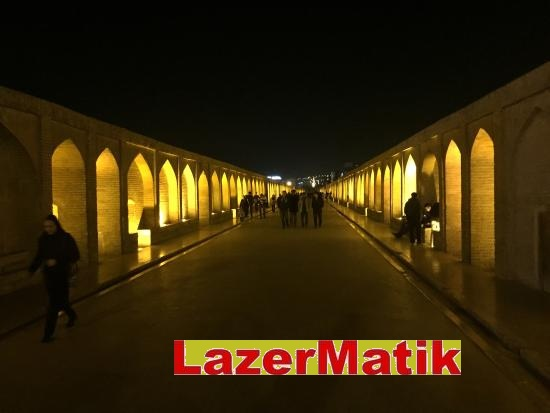
\includegraphics[width=25mm]{images/mt/synmetu1.jpg} &   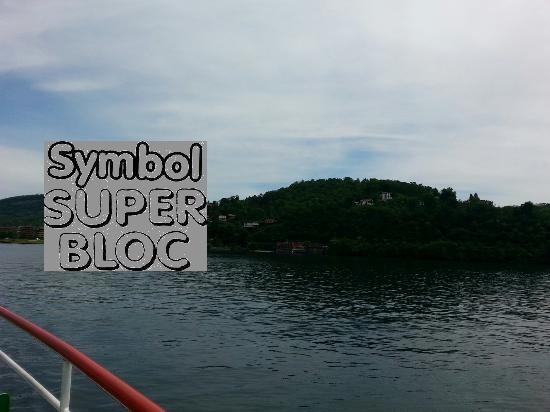
\includegraphics[width=25mm]{images/mt/synmetu2.jpg}  & 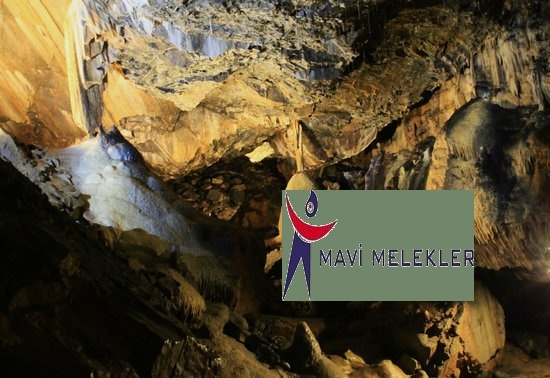
\includegraphics[width=25mm]{images/mt/synmetu3.jpg} &   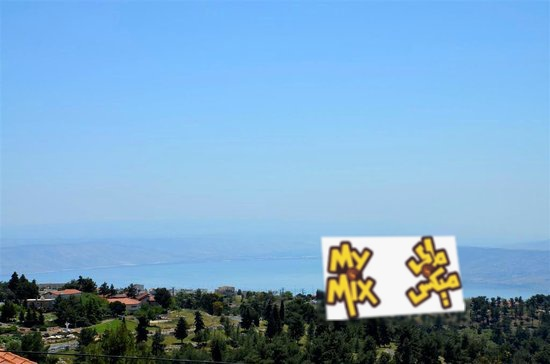
\includegraphics[width=25mm]{images/mt/synmetu4.jpg} \\
    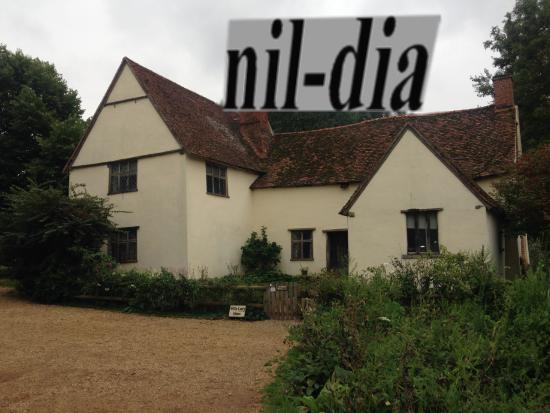
\includegraphics[width=25mm]{images/mt/synmetu5.jpg} &   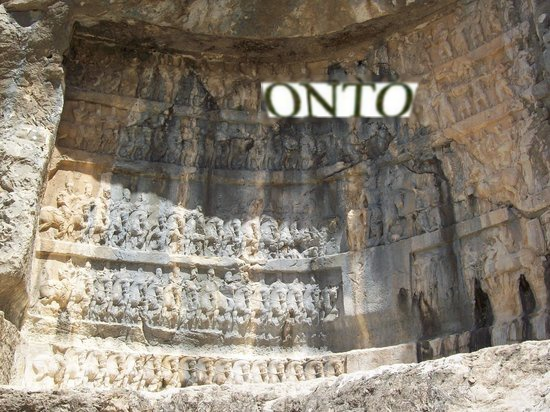
\includegraphics[width=25mm]{images/mt/synmetu6.jpg}  & 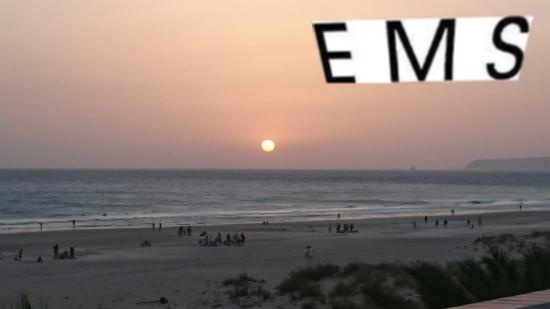
\includegraphics[width=25mm]{images/mt/synmetu7.jpg} &   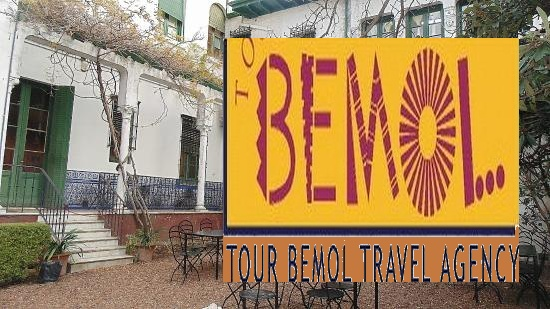
\includegraphics[width=25mm]{images/mt/synmetu8.jpg} 
\end{tabular}
\caption{Generated synthetic logo images}
\end{figure}

\iffalse

\begin{table}[ht!]
\centering
\caption{Applied transformations}
\label{table:logotransformations}
\begin{tabular}{|c|c|c|}
\hline & \textbf{Brightness adjustment} & \textbf{Hue rotation} \\
\hline
\textbf{33\%} & - & - \\
\hline
\textbf{33\%} & yes & yes \\
\hline
\textbf{33\%} & yes & yes \\ \hline
\end{tabular}
\end{table}

\fi






\section{Logo Detection}



\section{Logo Retrieval}
